\documentclass[sigconf,anonymous,review]{acmart}
\setcopyright{none}
\setlength{\emergencystretch}{2em}
\settopmatter{printacmref=false}
\renewcommand\footnotetextcopyrightpermission[1]{}
\acmConference[IAFM '26]{Workshop on Interpretability and Alignment of Financial Models}{November 2026}{Milan, Italy}
\acmYear{2026}
\title{When Portfolio Rewards Miss the Target: Exact Mismatch and Policy Alignment}
\author{Anonymous Author(s)}
\newcommand{\E}{\mathbb{E}}
\newcommand{\Var}{\operatorname{Var}}
\newcommand{\Cov}{\operatorname{Cov}}
\newcommand{\eq}{\mathrm{eq}}
\newtheorem{proposition}{Proposition}
\newtheorem{theorem}{Theorem}
\begin{document}
\begin{abstract}
A risk-sensitive portfolio reward need not implement the investor's stated objective. We examine this difference in two settings. For independent returns, we derive the exact leading policy discrepancy that remains after optimally calibrating a quadratic wealth-increment reward: a common scalar penalty cannot recover terminal mean--variance equilibrium when interest is nonzero and the horizon exceeds one period. For constrained allocation with turnover costs, the mean--variance auxiliary identity shows why risk and cost coefficients must be calibrated together. A walk-forward study evaluates 10, 30 and 49 US industry portfolios over 432 months, with a 17-setting robustness grid for ten industries. Joint calibration recovers the fitted policy; the unconstrained scalar correction worsens alignment in both larger universes. An adapted mean--variance policy iteration method also matches the ten-industry reference. Realised results favour minimum variance, and joint calibration underperforms the raw reward in the larger universes. The analysis separates the economic meaning of a reward from optimisation accuracy and investment performance, allowing each to be checked directly.
\end{abstract}
\ccsdesc[500]{Computing methodologies~Reinforcement learning}
\ccsdesc[300]{Applied computing~Economics}
\keywords{portfolio allocation, reward alignment, mean--variance, reinforcement learning, transaction costs}
\maketitle

\section{Introduction}
A portfolio mandate specifies a trade-off between return, risk and trading costs. A learning algorithm acts on a reward. These two descriptions need not select the same allocation: replacing variance with a second moment also penalises squared expected return, and correcting the risk coefficient alone can change the effective cost preference. Accurate reward optimisation can therefore implement a different mandate.

This problem sits alongside the estimation problem at the heart of portfolio choice. Markowitz~\cite{markowitz1952} separates beliefs about returns from decisions made using those beliefs. DeMiguel et al.~\cite{demiguel2009} show how estimation error can overwhelm the gains from optimal diversification. Neither better forecasts nor a stronger optimiser, however, repairs a reward that encodes a different preference. To identify which intervention is needed, the financial objective, the reward-induced optimum and the learned policy must be compared separately.

We make that comparison explicit. For a terminal mean--variance equilibrium benchmark, we derive the exact leading discrepancy remaining after the best common scalar calibration of a wealth-increment reward. Nonzero interest creates a policy difference that coefficient tuning cannot eliminate. For constrained allocation with turnover costs, we use the established MVPI mean auxiliary~\cite{zhang2021} to identify the cost distortion caused by risk-only calibration and construct a reference-preserving reward. The historical construction is a certificate based on a known target; MVPI supplies an existing way to compute that target without inserting it first.

The empirical test holds estimates and pre-trade holdings fixed while changing the reward. Ten-, thirty- and forty-nine-industry portfolios distinguish fitted alignment from realised investment performance. A finite-budget optimisation experiment further separates persistent reward-design error from learning error. These tests make a reward's financial meaning observable: they identify a discrepancy, quantify its consequence in the investor's objective, and check whether changing the coefficients removes it. They complement performance evaluation rather than replacing it.

\section{Related work and comparison design}
\paragraph{Portfolio choice and estimation risk.}
The mean--variance reference follows Markowitz~\cite{markowitz1952}, pp.\ 81--83. DeMiguel, Garlappi and Uppal~\cite{demiguel2009}, Tables 3--5, compare 14 allocation models with $1/N$ using Sharpe, certainty-equivalent return and turnover. Their Proposition 1 and Figure 1 relate estimation-window requirements to dimension and investment opportunities; they do not prescribe a minimum portfolio size. Their Table 2 and Appendix A.2 include ten industries plus the market. We retain equal weight as a substantive benchmark and extend the audit to finer industry classifications. Ledoit and Wolf~\cite{ledoit2017}, Section 4.3 and Table 1, evaluate nonlinear covariance shrinkage by its out-of-sample portfolio consequences. Their estimator addresses noisy inputs; our comparison holds inputs fixed to isolate reward semantics. Our fixed diagonal shrinkage is not their estimator.

\paragraph{Economic objectives and trading costs.}
G\^arleanu and Pedersen~\cite{garleanu2013}, Eq.\ (4) and Propositions 2--3, derive a dynamic policy balancing predictable returns, risk and quadratic trading costs. Their Table II compares commodity-futures strategies net of costs. Our rolling one-period target is a different object: it does not incorporate their continuation decisions. More recently, DeMiguel, Mart\'in-Utrera and Uppal~\cite{demiguel2024}, Eq.\ (6), optimise conditional multifactor MV net of costs. Their Table II reports improved out-of-sample performance over an unconditional portfolio, while Table III isolates the roles of cost-aware optimisation and netting trades. These results motivate treating cost preferences as part of the objective, not merely subtracting costs at evaluation. We test whether a reward transformation preserves that preference; we do not reproduce their factor strategy.

\paragraph{Objective-aware financial learning.}
Simon et al.~\cite{simon2026}, Section 4.1, Eq.\ (17), use centred MV utility with deep parametric portfolio policies; Section 3.6 treats turnover costs. Gollart and Okhrin~\cite{gollart2025}, Section 4.2.1, Table 1, use terminal utility and validate modified DDPG against an analytical Heston--Nandi benchmark. Chaouki et al.~\cite{chaouki2020}, Section 3, also compare learned and known controls. Known-policy validation and direct preference optimisation are established practices. Our additional result quantifies a particular surrogate's irreducible policy discrepancy after optimal scalar tuning.

\paragraph{Reward formulations.}
Jiang et al.~\cite{jiang2025}, Eq.\ (8), combine net log return and variance; Eq.\ (19) adds soft constraints to a DPG-based portfolio method. We adapt that preference to common monthly estimates, hard simplex constraints and a first-order turnover charge. Their architecture and stock-universe results are not reproduced. Jiang et al.~\cite{jiang2024}, Eq.\ (4), penalise variance and costs around portfolio value; their TD3/PPO/DDPG comparison motivates auditing both penalties. Cong et al.~\cite{cong2026}, Eqs.\ (19)--(20), instead permit differentiable trajectory objectives, including window Sharpe. Such preferences are legitimate alternatives, not automatically implementations of terminal MV.

\paragraph{Time consistency and equivalent objectives.}
Precommitment~\cite{ling2000} and equilibrium~\cite{basak2010,dai2023} answer different control questions. Czichowsky~\cite{czichowsky2013}, Lemma 3.2 of the inspected preprint, includes a continuation-covariance hedge. Bj\"ork et al.~\cite{bkm2016}, Propositions 8.1 and 10.2 of the long 2016 preprint, develop equivalent objectives and terminal-unit variance penalisation. MVPI~\cite{zhang2021} already contains the auxiliary transformation used below. Our theoretical contribution is the exact leading minimum discrepancy for the raw increment-reward family, rather than a claim to have introduced equivalent-objective methods.

\section{An exact test of terminal-objective alignment}
\subsection{Market, reference and discrepancy}
Consider independent excess returns $P_t\in\mathbb R^n$ with constant mean $m\ne0$ and positive definite covariance $\Sigma$. Wealth evolves as
\begin{equation}
 X_{t+1}=sX_t+P_t^\top u_t,\qquad X_0=x_0,
\end{equation}
with unrestricted risky dollar positions $u_t$ and constant gross risk-free return $s>0$. The terminal objective is $J=\E X_T-\varphi\Var X_T$, $\varphi>0$. The time-consistent equilibrium policy is
\begin{equation}
 u_t^\eq=\frac{\Sigma^{-1}m}{2\varphi H_t},\qquad H_t=s^{T-t-1}.
\end{equation}
It is not the initial-date precommitment maximiser. Define $M=\Sigma+mm^\top$, $d=M^{-1}m$, $\nu=m^\top d<1$ and $b=[2\varphi(1-\nu)]^{-1}$. The reward family is $r_t=\Delta X_t-\kappa(\Delta X_t)^2$, with one constant $\kappa>0$. Let $\pi^\kappa$ be its exact additive-reward optimum, and measure
\begin{equation}
 D^2=\sum_{t=0}^{T-1}\E_{\pi^\kappa}\|\pi^\kappa(t,X_t)-u_t^\eq\|^2.
\end{equation}
This is an occupancy-dependent discrepancy, not a symmetric policy metric.

\subsection{What scalar calibration cannot repair}
\begin{theorem}\label{th:mismatch}
For fixed $T\ge2$, as $s\to1$,
\begin{align}
 \min_{\kappa>0}D&=c_T|s-1|+O((s-1)^2),\\
 c_T&=\|d\|b\sqrt{\frac{T(T^2-1)}3+\frac{\nu(1-\nu)T(T-1)}2}.
\end{align}
At $s=1$ exact matching holds for $\kappa=\varphi(1-\nu)$. For $s\ne1$, $T\ge2$, exact matching along the surrogate occupancy is impossible.
\end{theorem}
\begin{proof}
Write the Bellman value $W_t(x)=p_tx^2+q_tx+c_t$, with $p_T=q_T=0$ and $g_t=\kappa(s-1)-sp_{t+1}$. Completing the square gives $u_t=\alpha_tx+\beta_t$ and
\begin{align}
 \alpha_t&=-\frac{dg_t}{\kappa-p_{t+1}},&
 \beta_t&=\frac{d(1+q_{t+1})}{2(\kappa-p_{t+1})},\\
 p_t&=\frac{\kappa p_{t+1}-(1-\nu)g_t^2}{\kappa-p_{t+1}},&
 1+q_t&=(1+q_{t+1})\left(s-\frac{\nu g_t}{\kappa-p_{t+1}}\right).
\end{align}
Induction gives $p_t\le0$, so the action Hessian is negative definite and these are global Markov optima. Set $e=s-1$, $h=(2\kappa)^{-1}$. The ratios $p_t/\kappa$ and $q_t$ are independent of $\kappa$, hence pathwise $X_t=L_t(e)x_0+hZ_t(e)$. Consequently $D^2=F(e,h)$ is exactly quadratic in $h$, with analytic coefficients near zero and $F(0,h)=T\|d\|^2(h-b)^2$. Its global minimiser is analytic and remains positive near zero.

Put $\kappa=\varphi(1-\nu)(1+we)$. The leading action difference is $de$ times
\[
 -X_t+b[(T-t-1)(2-\nu)-w].
\]
At $e=0$, $\E X_t=x_0+t\nu b$ and $\Var X_t=tb^2\nu(1-\nu)$. Minimisation yields $w^*=(T-1)(1-\nu)-x_0/b$. The centred means are $b(T-1-2t)$; summing their squares and variances gives the displayed $c_T^2$. Analyticity then gives the stated remainder after taking square roots.

Finally, matching at the first date forces a nonzero equilibrium action and positive subsequent wealth variance. At the final date the surrogate has slope $-d(s-1)$ whereas equilibrium is constant. Almost-sure equality is impossible when $s\ne1$.
\end{proof}
The coefficient grows as $T^{3/2}$ for large $T$, but the expansion is for fixed $T$; no uniform joint interest--horizon limit is claimed. The obstruction concerns this reward family, not all additive objectives.

\subsection{A reference-preserving reward}
Allow moments to vary by date while returns remain independent. Define $Y_t=H_tP_t^\top u_t$ and use
\begin{equation}\label{eq:design}
 r_t^{\rm design}=Y_t-\varphi(1-\nu_t)Y_t^2.
\end{equation}
The expected reward is strictly concave. Its maximiser is
\[u_t=\frac{\Sigma_t^{-1}m_t}{2\varphi H_t}.\] Future rewards admit state-independent maximisers, so backward induction recovers the equilibrium. This construction specialises the equivalent-objective approach of Bj\"ork et al.\ \cite{bkm2016} and changes the optimum of the original raw reward. Dependent returns require continuation terms, so Eq.\ \eqref{eq:design} is not applied as a historical multiperiod theorem.

\begin{figure}[t]
\centering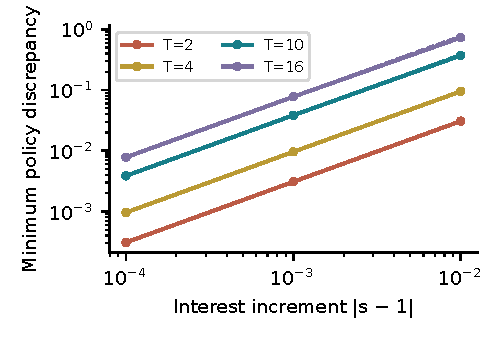
\includegraphics[width=\columnwidth]{figures/theory.pdf}
\caption{Exact minimum discrepancy (points and solid lines) and local prediction $c_T|s-1|$ (dashed lines). Here $x_0=\varphi=1$, $m=(.06,.04,.02)$, volatilities $(.18,.12,.08)$, and correlations $(\rho_{12},\rho_{13},\rho_{23})=(.30,-.10,.05)$. This concerns terminal equilibrium, not the fitted historical reference.}
\Description{Log-log plot comparing exact discrepancy with the local formula for four horizons.}
\label{fig:theory}
\end{figure}

\section{Constrained alignment with turnover costs}
Historical implementation adds constraints and costs. On a fixed past-only estimated state, let $C$ be the simplex, $p$ the pre-trade allocation and $c(u)=\|u-p\|_1$. Define the fitted one-period preference
\begin{equation}\label{eq:target}
 F(u)=m^\top u-\varphi u^\top\Sigma u-\lambda c(u),\quad u\in C.
\end{equation}
Its unique optimum $u^*$ is a \emph{fitted reference}, not the unknown true market optimum. This section does not extend Theorem~\ref{th:mismatch} to estimated or dependent markets.

\begin{proposition}\label{prop:joint}
Let $y^*=m^\top u^*$ and $A=1+2\varphi y^*>0$. The second-moment reward objective
\begin{equation}
 Q(u)=m^\top u-\frac{\varphi}{A}u^\top M u-\frac{\lambda}{A}c(u)
\end{equation}
has the same unique maximiser as $F$.
\end{proposition}
\begin{proof}
For all feasible $u$,
\begin{equation}\label{eq:identity}
 AQ(u)=F(u)-\varphi(m^\top u-y^*)^2+\varphi(y^*)^2.
\end{equation}
At $u^*$ the square vanishes and $F$ is maximal. Since $A>0$, the assertion follows.
\end{proof}
The argument applies to any feasible set with a global maximiser. Convexity and positive definite covariance ensure uniqueness here. The identity follows the mean auxiliary used in MVPI\ \cite{zhang2021}.

If only the risk coefficient is divided by $A$, while the cost coefficient stays $\lambda$, the right-hand side of Eq.\ \eqref{eq:identity} gains the extra term
\begin{equation}\label{eq:costdistortion}
 -2\varphi y^*\lambda c(u).
\end{equation}
When $y^*>0$, this increases the effective cost preference. It need not imply monotone realised turnover on the strategy's evolving path. The unconstrained formula $\varphi(1-\nu)$ likewise need not calibrate a constrained optimum.

Joint calibration uses $u^*$ and therefore serves as a certificate of alignment with a known reference. As a constructive prior-art comparator, we also alternate maximising
\begin{equation}
 (1+2\varphi y)m^\top u-\varphi u^\top Mu-\lambda c(u)
\end{equation}
and setting $y=m^\top u$. This is an adaptation of the MVPI mean auxiliary to the constrained one-period problem. Including the term $-\varphi y^2$ gives a jointly strictly concave objective, since its quadratic block has Schur complement $\Sigma\succ0$. Exact block updates converge to the same target. This provides a constructive comparator with the same optimum.

\section{Historical study}
\subsection{Data and protocol}
The primary study uses Kenneth French's ten value-weighted US industry portfolio monthly total returns and the Fama--French risk-free series\ \cite{french}. The archived downloads have a recorded SHA-256 manifest. Estimation data start January 1970; evaluation covers January 1990--December 2025 (432 months). This is a retrospective study on the August 2026 revised vintage, not a point-in-time constituent dataset. Industry portfolios are research portfolios, not directly tradeable funds; their internal reconstruction costs are not included. The provider's CRSP processing and risk-free source changes also form part of this data vintage.

For month $t$, use only the previous 120 months of excess returns to estimate $m$ and the unbiased covariance, shrunk 10\% toward its diagonal. All strategies are long-only and fully invested. The primary settings are $\varphi=5$ and $\lambda=0.001$ (10 basis points per unit of L1 turnover). Pre-trade weights drift with realised gross asset returns. Net portfolio return uses the explicit first-order convention $u_t^\top R_t-\lambda\|u_t-p_t\|_1$, not a market-impact model or exact intramonth execution equation. The experimental protocol fixed these choices before strategy outcomes were inspected.

\subsection{Comparators and measurements}
We solve the covariance-MV target, raw second moment ($\kappa=\varphi$), unconstrained scalar calibration ($\kappa=\varphi(1-\nu)$), reference-based risk-only calibration, joint calibration, and MVPI adaptation. Equal weight and minimum variance provide conventional portfolio controls. Log utility and log-minus-variance adapt the reward preference in Jiang et al.\ \cite{jiang2025}; every method uses the same monthly data and feasible set. The comparison tests induced preferences under common estimates, not which published learning architecture is best.

For alignment, all methods face the target strategy's \emph{same pre-trade state}. We report Euclidean allocation distance and fitted regret $F(u^*)-F(u)$. Each strategy also follows its own pre-trade states for realised performance. This avoids conflating state divergence with the local reward comparison. Quadratic solutions have independent linear-programme first-order certificates; the largest saved common-state certificate is $4.27\times10^{-9}$ in objective units. The observed agreement of calibrated policies is considerably tighter than the acceptance tolerance.

Realised metrics are monthly excess-return MV, annualised excess Sharpe, return, volatility, turnover and drawdown. Uncertainty for paired MV differences uses 1,000 circular moving-block bootstrap resamples, blocks of 12 months, seed 8128. These intervals describe the observed strategy-return sequences, not full estimator-refitting or model-selection uncertainty. Robustness spans 17 prespecified combinations: $\varphi\in\{2,5,10\}$ and cost $\{0,10,25\}$ bp at the primary estimator, plus windows $\{60,120,240\}$ and covariance shrinkage $\{0,0.1,0.5\}$ at the primary preferences. The overlapping primary case is counted once.

\begin{table*}[t]
\centering
\caption{Reward-formulation comparison on historical data, 1990--2025. Published rewards are adapted to a common environment; complete published algorithms are not reproduced. Bold identifies our joint-calibration construction, not the best realised performance. Distance and fitted regret use common states; realised metrics use each strategy's own path. Gap and MV score are monthly basis-point units.}
\label{tab:historical}
\begin{tabular}{@{}p{.23\textwidth}p{.24\textwidth}rrrr@{}}\toprule
Method & Source / role & \shortstack{Allocation\\distance} & \shortstack{Fitted gap\\(bp)} & \shortstack{Excess\\Sharpe} & \shortstack{Realised MV\\(bp)}\\\midrule
Target & Markowitz (1952) & 0.00000 & 0.0000 & 0.570 & -8.497 \\
Minimum variance & Markowitz (1952) & 0.23843 & 9.0252 & 0.645 & 5.274 \\
Equal weight & DeMiguel et al. (2009) & 0.43495 & 46.2626 & 0.622 & -11.893 \\
MVPI adaptation & Zhang et al. (2021) & 0.00000 & 0.0000 & 0.570 & -8.497 \\
Log minus variance & Jiang et al. (2025) & 0.01286 & 0.0287 & 0.572 & -7.123 \\
Log utility & Log-utility control (2026) & 0.54848 & 39.7855 & 0.344 & -133.295 \\
Raw second moment & Uncalibrated baseline (2026) & 0.00843 & 0.0148 & 0.573 & -7.182 \\
Unconstrained scalar & Analytical baseline (2026) & 0.00540 & 0.0043 & 0.568 & -8.882 \\
Risk-only calibration & Calibration ablation (2026) & 0.00510 & 0.0033 & 0.571 & -8.365 \\
\midrule
\textbf{Joint calibration (ours)} & \textbf{This study (2026)} & \textbf{0.00000} & \textbf{0.0000} & \textbf{0.570} & \textbf{-8.497} \\
\bottomrule\end{tabular}

\par\smallskip
\parbox{\textwidth}{\footnotesize\emph{Sources:} mean--variance foundation~\cite{markowitz1952}; equal-weight benchmark~\cite{demiguel2009}; log-minus-variance reward~\cite{jiang2025}; MVPI~\cite{zhang2021}. For controls and calibration constructions, 2026 denotes this study's implementation, not the historical origin of the method.}
\end{table*}

\subsection{Results}
Table~\ref{tab:historical} shows that raw second-moment optimisation has mean allocation distance 0.00843. Unconstrained scalar calibration reduces this to 0.00540; reference-based risk-only calibration retains 0.00510. Joint calibration and MVPI agree with the fitted reference to numerical precision. The adapted log-minus-variance objective has distance 0.01286; log utility alone is much farther away. The differences measure departure from the specified MV preference; log utility represents a different investment objective.

Across all 17 settings, the largest mean joint-calibration distance is $1.54\times10^{-7}$; raw mean distances range from 0.00157 to 0.03682. Thus constraints and trading costs do not break the joint identity, while unconstrained scalar calibration is not a universal repair. Figure~\ref{fig:historical} relates alignment to historical outcomes, and Figure~\ref{fig:robust} gives robustness and uncertainty.

In the ten-industry primary study, joint calibration has realised monthly MV lower than raw by 1.315 bp, with 95\% interval $[-3.318,0.343]$ bp. Against scalar calibration the difference is 0.385 bp. Its interval is $[-0.570,1.351]$ bp. Against risk-only calibration the difference is $-0.131$ bp, with interval $[-0.889,0.634]$ bp. All three primary intervals include zero. Minimum variance has both a better realised MV score and higher Sharpe than the fitted target in the primary sample. This illustrates estimation risk: precise implementation of estimated preferences cannot guarantee the best realised allocation. Equal weight has higher Sharpe than the target but lower realised MV, so Sharpe ranking alone does not answer even the ex-post MV comparison.

\begin{figure*}[p]
\centering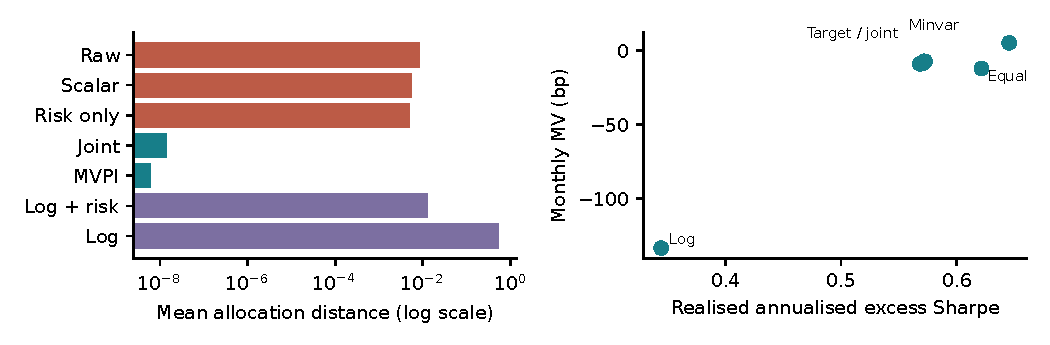
\includegraphics[width=.94\textwidth]{figures/historical.pdf}
\caption{Left: mean common-state allocation distance; the logarithmic axis exposes numerical agreement for joint calibration and MVPI. Right: realised Sharpe and monthly MV need not rank policies alike. Equal weight has higher Sharpe but lower MV than the fitted target.}
\Description{Allocation distances on the left and realised Sharpe versus mean-variance on the right.}
\label{fig:historical}
\end{figure*}
\begin{figure*}[p]
\centering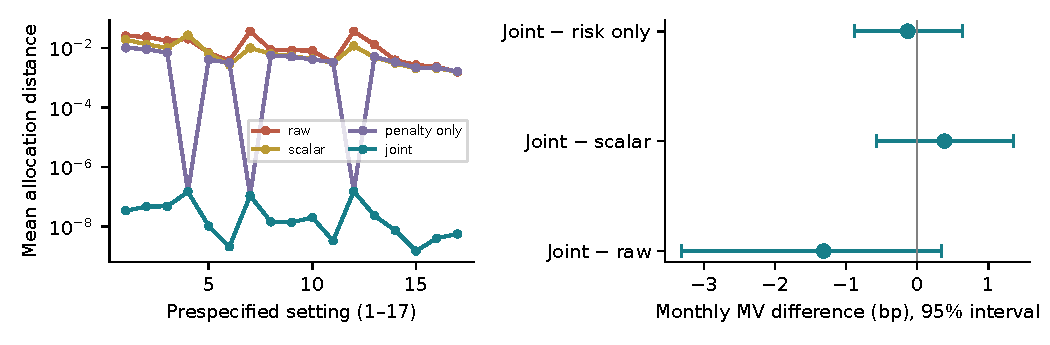
\includegraphics[width=.94\textwidth]{figures/robustness.pdf}
\caption{Left: alignment across the 17 prespecified settings, ordered by window, risk penalty, cost and shrinkage. Right: paired 12-month-block bootstrap intervals all include zero. Exact fitted alignment does not imply a statistically clear realised MV advantage.}
\Description{Seventeen-setting allocation-distance curves and three paired confidence intervals crossing zero.}
\label{fig:robust}
\end{figure*}

\subsection{Portfolio dimension and estimation risk}
The dimension extension uses French's 30- and 49-industry portfolios, preserving the August 2026 vintage, 120-month window, 432 evaluation dates, constraints and cost settings. It follows a protocol fixed before these additional outcomes were inspected. The seven quadratic/control methods are rerun; the MVPI and log comparators remain in the ten-industry primary comparison. The ratios $N/L$ rise from 0.083 to 0.250 and 0.408. The respective mean/covariance entry counts are 65, 495 and 1,274, illustrating the larger estimation burden. None of these settings has $N>L$.

DeMiguel et al.~\cite{demiguel2009}, Proposition 1, show why dimension must be considered jointly with estimation length and investment opportunities. Their frequently cited 3,000/6,000-month requirements are model-calibrated examples, not universal thresholds. Their ten-industry dataset justifies retaining a compact primary benchmark; the finer classifications test whether the alignment result survives a larger decision space. Different industry aggregations preclude a causal interpretation of dimension alone.

Table~\ref{tab:dimension} shows joint calibration at numerical agreement in all three universes. By contrast, unconstrained scalar calibration increases mean distance from 0.01852 to 0.02183 for 30 industries and from 0.02079 to 0.05354 for 49. Its fitted gap also increases. A scalar rule derived without constraints can thus be worse than leaving the penalty uncalibrated. Joint calibration addresses this particular specification error but not estimation risk: its realised MV is below raw by 5.216 and 5.670 monthly bp in the two added universes. Their paired 95\% intervals are $[-10.044,-0.903]$ and $[-10.747,-0.882]$ bp. These are descriptive, unadjusted comparisons of overlapping strategy-return paths. Minimum variance has the highest realised MV among the seven tested methods in each universe; joint versus $1/N$ intervals include zero throughout.

\begin{table*}[t]
\centering
\caption{Dimension robustness under the same 120-month estimation window, 1990--2025 evaluation and transaction costs. Each cell lists results for $N=10/30/49$. Distances and fitted gaps use common states; realised MV uses own-state net excess returns. Bold identifies our construction. Values below $10^{-8}$ bp in magnitude are reported as zero.}
\label{tab:dimension}
\begin{tabular}{@{}lrrr@{}}\toprule
Method & Allocation distance & Fitted gap (bp) & Realised MV (bp)\\\midrule
Fitted MV target & 0.00000 / 0.00000 / 0.00000 & 0.0000 / 0.0000 / 0.0000 & -8.497 / -26.096 / -30.567 \\
Equal weight ($1/N$) & 0.43495 / 0.42122 / 0.40647 & 46.2626 / 82.8426 / 94.3835 & -11.893 / -31.669 / -30.592 \\
Minimum variance & 0.23843 / 0.33760 / 0.35794 & 9.0252 / 21.0178 / 28.1249 & 5.274 / -0.416 / -4.808 \\
Raw second moment & 0.00843 / 0.01852 / 0.02079 & 0.0148 / 0.0803 / 0.1182 & -7.182 / -20.880 / -24.897 \\
Unconstrained scalar & 0.00540 / 0.02183 / 0.05354 & 0.0043 / 0.1099 / 0.7043 & -8.882 / -31.275 / -40.094 \\
Risk-only calibration & 0.00510 / 0.00758 / 0.00820 & 0.0033 / 0.0067 / 0.0081 & -8.365 / -25.660 / -30.064 \\
\midrule
\textbf{Joint calibration (ours)} & $\mathbf{1.40\times10^{-8}}$ / $\mathbf{7.33\times10^{-8}}$ / $\mathbf{1.29\times10^{-7}}$ & \textbf{0.0000 / 0.0000 / 0.0000} & \textbf{-8.497 / -26.096 / -30.567} \\
\bottomrule\end{tabular}

\end{table*}

\subsection{Separating optimisation from reward design}
A finite-budget experiment assigns independent softmax policy logits to each of the 432 historical common states. Adam uses learning rate 0.05, initial logits $N(0,0.1^2)$, five matched seeds and 50, 250, 1,000 and 5,000 gradient steps. Each objective uses only its state's lagged estimates. Independent logits isolate optimisation error on each fitted state. They do not test generalisation across states, as a predictive neural policy would.

Let $u_r$ maximise the specified reward and $\widehat u_r$ be the finite-budget allocation. We report the nonnegative own-reward optimisation gap separately from
\begin{align}
 F(u^*)-F(\widehat u_r)
 &= [F(u^*)-F(u_r)]\nonumber\\
 &\quad+[F(u_r)-F(\widehat u_r)].
\end{align}
The second bracket is a \emph{signed} target-value difference; it is not the own-reward optimisation gap. At 5,000 steps, mean own-reward optimisation gaps remain approximately $4\times10^{-6}$, exceeding the exact raw design gap of $1.48\times10^{-6}$. Thus finite-budget error can dominate the reward discrepancy. Figure~\ref{fig:learning} shows why these must be kept separate: improving the raw-reward optimiser does not remove its exact design gap. The target and joint reward have the same limiting optimum but can exhibit different finite-budget trajectories because their objective geometries differ.

\begin{figure*}[p]
\centering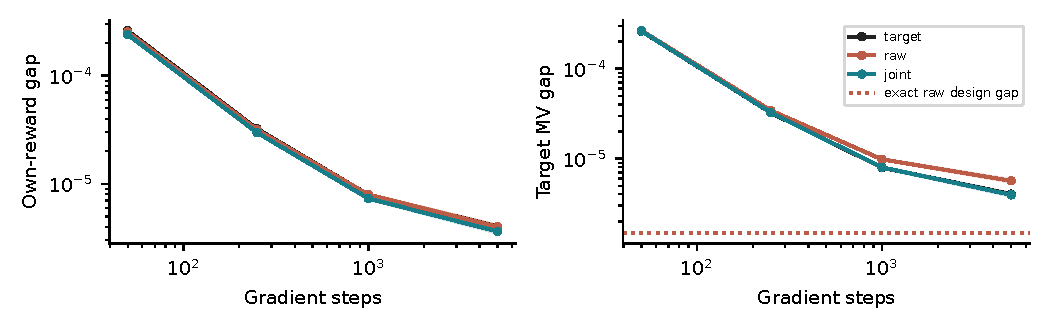
\includegraphics[width=.94\textwidth]{figures/learning.pdf}
\caption{Finite-budget softmax optimisation on historical fitted states. Lines are five-seed means, shading the seed range. Left uses each method's own reward; right uses the common MV target. The dotted line is the exact raw reward-design gap. This diagnostic measures optimisation accuracy, not generalisation.}
\Description{Own-reward and target gaps decline with gradient steps; the raw target gap remains above its design floor.}
\label{fig:learning}
\end{figure*}

\section{Reproducible portfolio comparisons}
\subsection{Estimates and portfolio accounting}
For $N\in\{10,30,49\}$, let $X_s=R_s-r_{f,s}\mathbf1$ and use only $t-L\le s<t$. Set
\begin{align}
 m_t&=L^{-1}\sum_s X_s,\qquad
 S_t=(L-1)^{-1}\sum_s(X_s-m_t)(X_s-m_t)^\top,\\
 \Sigma_t&=(1-h)S_t+h\operatorname{diag}(S_t).
\end{align}
The primary estimator uses $L=120$, $h=0.1$ and no mean shrinkage. Percent returns are converted to decimals. Within 1970--2025, missing sentinels, duplicate or absent months are rejected. Earlier missing industries in the 49-industry file are excluded by the date boundary, not imputed. All decisions use the preceding window.

At the common reference holdings $p_t^*$, each method supplies $u_t^r$ for the alignment statistics $d_t^r=\|u_t^r-u_t^*\|_2$ and $g_t^r=F_t(u_t^*)-F_t(u_t^r)$. For investment evaluation it solves again at its own holdings $p_t^r$, giving $\bar u_t^r$. The net return is $(\bar u_t^r)^\top R_t-\lambda\|\bar u_t^r-p_t^r\|_1$, and relative holdings drift as
\begin{equation}
 p_{t+1,i}^r=\frac{\bar u_{t,i}^r(1+R_{t,i})}{1+(\bar u_t^r)^\top R_t}.
\end{equation}
All methods start equally weighted. Costs are subtracted separately under the first-order convention. Common-state comparisons isolate the local reward effect; own-state paths include consequences of earlier decisions.

\subsection{Published formulations under common information}
The MVPI adaptation alternates the auxiliary update $y\leftarrow m^\top u$ with the constrained portfolio step, keeping the original cost coefficient. It starts at $y=0$ and stops at a change below $10^{-10}$, within 200 iterations. Unlike reference-based joint calibration, it computes the target without first supplying it.

The Jiang et al.~\cite{jiang2025} adaptation maximises
\begin{equation}
 L^{-1}\sum_{s=t-L}^{t-1}\log(1+u^\top R_s)
 -\varphi u^\top\Sigma_tu-\lambda\|u-p_t\|_1.
\end{equation}
Zero variance penalty gives log utility. These use total returns; MV uses excess returns. Hard simplex constraints and linear costs replace the source paper's soft restrictions and log cost factor. This compares preferences under identical information, not published architectures or returns.

The minimum-variance control drops the estimated mean from $F$ while keeping its risk scaling and cost charge. Equal weight rebalances to $1/N$. Both test realised consequences beyond fidelity to the fitted target. Appendix~\ref{app:verification} gives solver certificates and uncertainty calculations.

\section{Financial semantics and model validation}
\subsection{Interpreting a decision through its objective}
An allocation can be explained by the financial preference it implements. In Eq.\ \eqref{eq:costdistortion}, risk-only calibration has a specific interpretation: after normalising the linear return coefficient, the investor faces an additional turnover penalty $2\varphi y^*\lambda$. This explanation predicts a change in the optimisation problem and can be tested by correcting the cost coefficient. It is a statement about the decision rule, not a narrative inferred from a favourable backtest.

The terminal benchmark identifies another mechanism: the raw reward introduces wealth dependence absent from the equilibrium allocation. Theorem~\ref{th:mismatch} quantifies why scalar tuning cannot remove this difference; changing to terminal units changes the reward family.

\subsection{A controlled test of policy fidelity}
Holding the estimated moments, constraints and pre-trade holdings fixed makes the comparison a controlled intervention on the reward. Allocation distance measures the decision change; fitted regret expresses its importance in the investor's objective. In the ten-industry experiment, the raw distance is 0.00843, but its fitted loss is only 0.0148 monthly basis points. Reporting both prevents a visible policy difference from being mistaken for a large economic loss.

This test can validate an RL reward before interpreting a learned policy. An exact or certified optimum supplies a reference for what training is trying to achieve. The softmax experiment tests whether reward design or incomplete optimisation dominates at a given budget. Own-reward error and the signed target-value transfer term remain distinct.

\subsection{What the audit establishes about model risk}
A reward can faithfully implement an estimated preference even when the estimates produce poor investment decisions. The dimension experiment makes that distinction concrete: changing the opportunity set can worsen realised outcomes without invalidating the calibration identity. The $1/N$ and minimum-variance controls expose this estimation risk, following the evaluation discipline of DeMiguel et al.~\cite{demiguel2009}. Conversely, a good realised return does not certify that the requested preference was implemented.

For model validation, the useful output is a reproducible record of the intended objective, induced allocation, numerical certificate and consequence of a specified reward correction. Such records support financial-semantic interpretation and faithful evaluation across market states and portfolio dimensions. They do not explain internal neural representations or establish that users understand a model better; those would require separate interpretability studies. When a tractable target already exists, it may be used directly. The calibration construction is useful for checking a surrogate or a learning implementation against that target, not as a computational shortcut over solving it.

\section{Conclusion}
The exact leading mismatch coefficient establishes a limit to scalar reward tuning for independent returns and unrestricted dollar positions. The constrained calibration identity instead concerns a fitted one-period objective. Across three industry universes, joint calibration removes its reward discrepancy, while an unconstrained scalar rule can worsen alignment. Better fitted alignment does not establish better investment performance: the larger-universe realised results favour the raw reward over the calibrated target.

The resulting audit distinguishes a reward's financial meaning from estimation and optimisation quality. It can test whether a portfolio learner implements the preference it was given, identify a coefficient-level correction and assess that correction separately on realised data. The historical study does not identify a true dependent-return terminal equilibrium. Continuation hedges, point-in-time investable universes and generalising neural policies require richer benchmarks.

\bibliographystyle{ACM-Reference-Format}
\bibliography{references}
\appendix
\twocolumn[{
\section*{Appendix}
\section{Complete robustness results}\label{app:robustness}
Table~\ref{tab:fullrobust} reports all 17 saved specifications underlying Figure~\ref{fig:robust}. Each row averages Euclidean allocation distance over the same 432 historical months. These are repeated specifications on one dataset, not independent samples. The primary setting is $L=120$, $\varphi=5$, $\lambda=10$ bp and $h=0.1$. The three columns isolate an uncalibrated reward, calibration of risk alone, and joint calibration of risk and costs.

\begin{center}
\captionof{table}{Complete common-state alignment results. $L$ is the estimation window in months, $\lambda$ is the cost per unit of L1 turnover in basis points, and $h$ is diagonal covariance shrinkage. Distances are weight-vector norms, not returns. Bold identifies joint calibration (ours).}
\label{tab:fullrobust}
\begin{tabular}{rrrrrrr}\toprule
$L$ & $\varphi$ & $\lambda$ (bp) & $h$ & Raw distance & Risk-only distance & \textbf{Joint (ours)}\\\midrule
60 & 5 & 10 & 0 & 0.02541 & 0.01018 & $\mathbf{3.44\times10^{-8}}$ \\
60 & 5 & 10 & 0.1 & 0.02391 & 0.00921 & $\mathbf{4.73\times10^{-8}}$ \\
60 & 5 & 10 & 0.5 & 0.01747 & 0.00698 & $\mathbf{4.80\times10^{-8}}$ \\
\midrule
120 & 2 & 0 & 0.1 & 0.02032 & 0.00000 & $\mathbf{1.48\times10^{-7}}$ \\
120 & 2 & 10 & 0.1 & 0.00697 & 0.00411 & $\mathbf{1.06\times10^{-8}}$ \\
120 & 2 & 25 & 0.1 & 0.00376 & 0.00320 & $\mathbf{2.10\times10^{-9}}$ \\
120 & 5 & 0 & 0.1 & 0.03664 & 0.00000 & $\mathbf{1.11\times10^{-7}}$ \\
120 & 5 & 10 & 0 & 0.00874 & 0.00566 & $\mathbf{1.45\times10^{-8}}$ \\
120 & 5 & 10 & 0.1 & 0.00843 & 0.00510 & $\mathbf{1.40\times10^{-8}}$ \\
120 & 5 & 10 & 0.5 & 0.00822 & 0.00413 & $\mathbf{2.02\times10^{-8}}$ \\
120 & 5 & 25 & 0.1 & 0.00324 & 0.00335 & $\mathbf{3.34\times10^{-9}}$ \\
120 & 10 & 0 & 0.1 & 0.03682 & 0.00000 & $\mathbf{1.54\times10^{-7}}$ \\
120 & 10 & 10 & 0.1 & 0.01296 & 0.00513 & $\mathbf{2.35\times10^{-8}}$ \\
120 & 10 & 25 & 0.1 & 0.00394 & 0.00338 & $\mathbf{7.45\times10^{-9}}$ \\
\midrule
240 & 5 & 10 & 0 & 0.00271 & 0.00219 & $\mathbf{1.51\times10^{-9}}$ \\
240 & 5 & 10 & 0.1 & 0.00237 & 0.00218 & $\mathbf{4.09\times10^{-9}}$ \\
240 & 5 & 10 & 0.5 & 0.00157 & 0.00165 & $\mathbf{5.71\times10^{-9}}$ \\
\bottomrule\end{tabular}
\end{center}
}]


\section{Numerical verification and uncertainty}\label{app:verification}
Quadratic objectives are solved with auxiliary variables $z_i\ge |u_i-p_i|$ and simplex constraints. The implemented minimisation is scaled for numerical conditioning, but certificates are computed in the original objective units. Given a feasible iterate $x$ in the extended polytope $\mathcal P$, a separate linear programme gives the certificate
\begin{equation}
 C(x)=\max_{v\in\mathcal P}\nabla f(x)^\top(x-v),
\end{equation}
where $f$ is the convex negative reward. Convexity implies $f(x)-\min f\le C(x)$. This checks accuracy independently of the quadratic optimiser's success flag. Poorly certified iterates are retried at different scales and rejected if the certificate remains above $2\times10^{-7}$. The log comparators use a separate concave optimisation problem; the quadratic certificate is not claimed for them.

Realised monthly MV is the sample mean of net excess returns minus $\varphi$ times their sample variance. Excess Sharpe annualises the monthly mean-to-standard-deviation ratio by $\sqrt{12}$. These are evaluated on each strategy's complete own-state return path. For paired MV uncertainty, the same circular 12-month blocks are sampled for both strategies, with 1,000 repetitions and seed 8128. Shared blocks retain contemporaneous dependence between strategies and some serial dependence within each path. The intervals condition on the fitted strategies' realised paths: they do not repeat estimation, select hyperparameters or quantify every source of model uncertainty.


\paragraph{Dimension-extension checks.}
Independent reconstruction of all 9,072 saved quadratic/control decisions across the three universes verifies lagged dates, simplex feasibility, drift, turnover, net returns and fitted gaps. Maximum absolute discrepancies are below $3\times10^{-16}$; the calibration identity residual is below $8\times10^{-18}$. Joint minus $1/N$ realised monthly MV is 3.396, 5.574 and 0.025 bp for $N=10,30,49$, with respective path-bootstrap intervals $[-16.646,24.172]$, $[-28.012,35.458]$ and $[-35.583,31.953]$ bp. These intervals do not establish superiority over naive diversification.

\end{document}
